% !TEX root = ../prospector.tex

\begin{figure}[t]
\centering
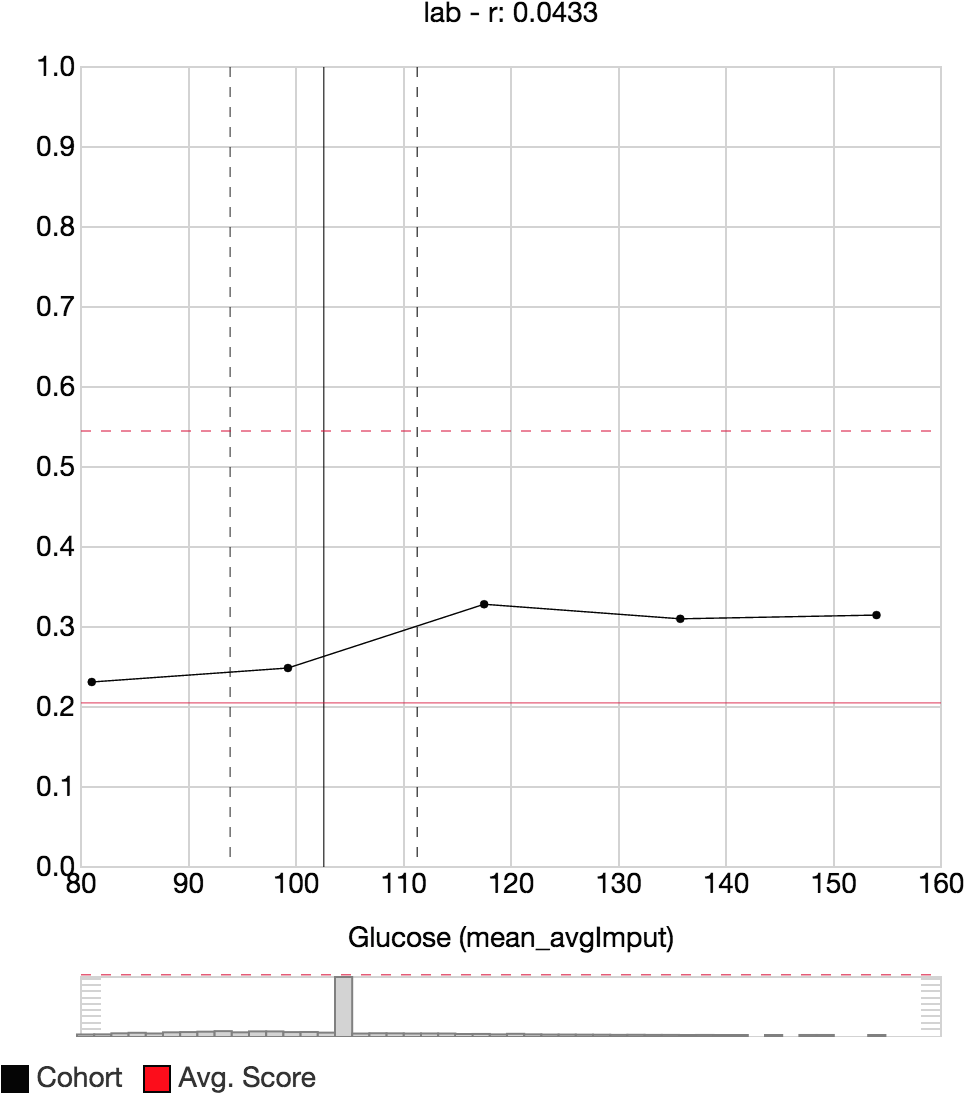
\includegraphics[width=0.3\textwidth]{prospector/sampling_1} % 0.3
~
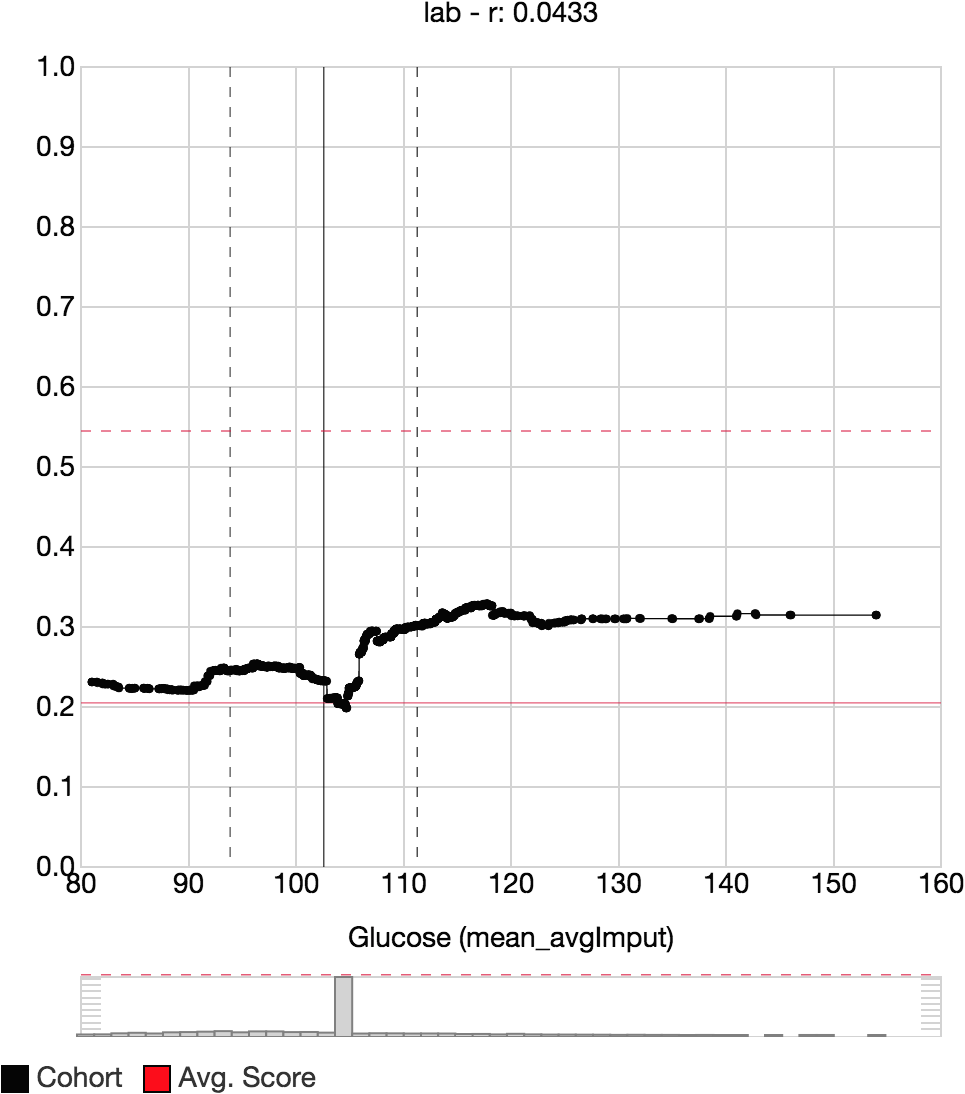
\includegraphics[width=0.3\textwidth]{prospector/sampling_2} % 0.3
~
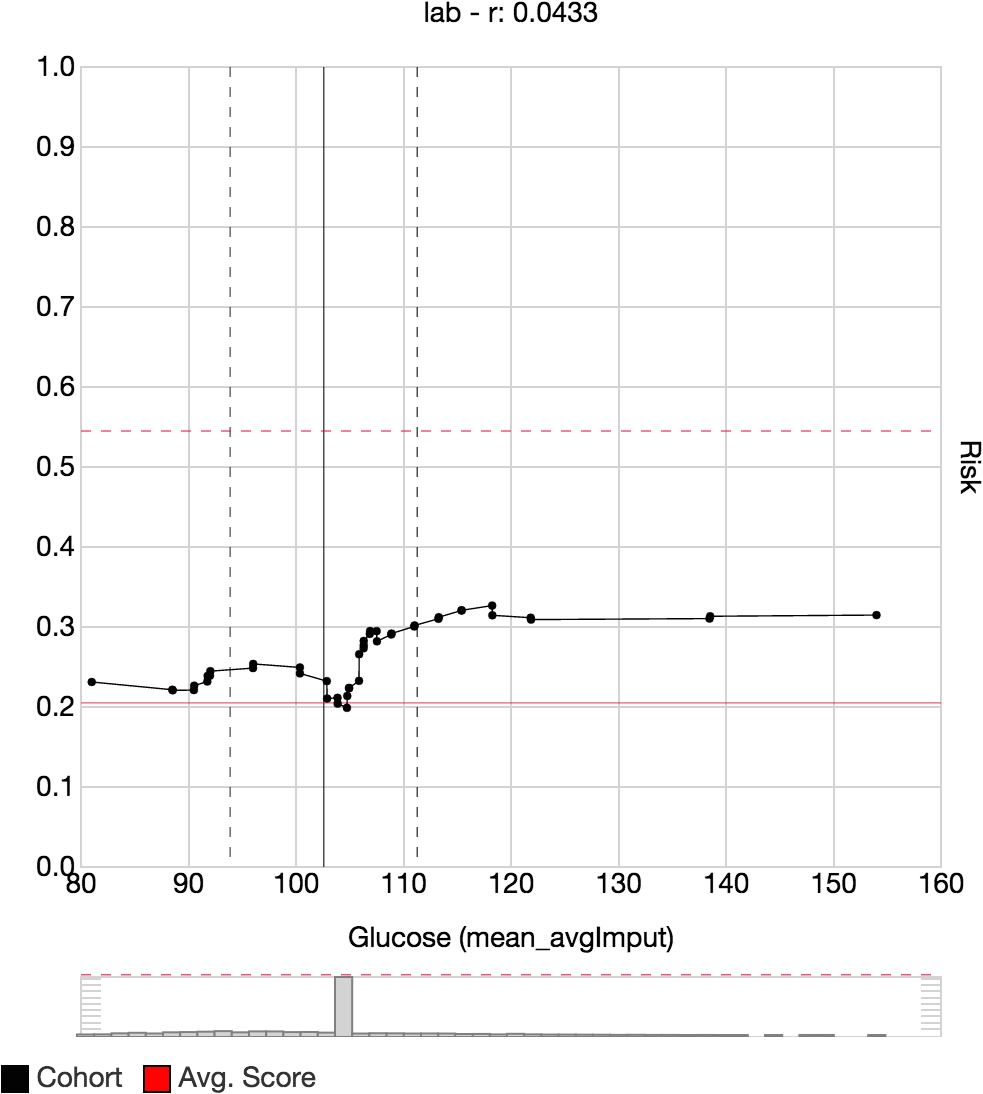
\includegraphics[width=0.3\textwidth]{prospector/sampling_3} % 0.3
\caption[Different sampling strategies for partial dependence plots.]{
Different sampling strategies for partial dependence plots.
The leftmost plot uses a na\"ive sampling which misses the
dip in the predicted risk for a Glucose value around 105.
Using the thresholds of the trees in the random forest
the middle plot shows all details of the displayed model.
The rightmost plot simplifies this by detecting co-linear points
and summarizing them into lines improving readability.
The dip in the predicted risk is due to imputation of missing values
to the mean of the observed values.
This increase in local noise shifts the prediction towards the overall
average predicted risk (the horizontal red line).
Most patients have never had their Glucose value measured.
}
\label{figs:sampling}
\end{figure}

\section{System}
In order to integrate partial dependence and localized inspection into our pipeline we propose
\prospector, a web-based interface.  The server side of \prospector can load any machine learning model accessible via python, or integrate with existing predictive modeling pipelines such as PARAMO \cite{paramo}.
% This can be done via a special admin page in the UI which also allows to
% precompute some partial dependence plots.
Although this paper demonstrates the system on clinical data, the tool is able to handle predictive models for other domains.  For example, the tool has also been used with exploring models that predict real estate prices, as well as classic data sets from the UCI Machine Learning Repository \cite{Lichman:2013}.

In this section, we first describe \prospector's novel enhancements of partial dependence plots.  Then, we describe how \prospector leverages partial dependence to support localized inspection.  Finally, we describe the workflow of how these techniques are integrated into \prospector's UI.
\subsection{Partial Dependence Plots}

Partial dependence is typically visualized as a partial dependence plot, which is a line graph that plots the fixed values for the target feature on the horizontal axis, and the corresponding predicted risk (probability of a certain outcome) on the vertical axis.  In \prospector, we enhance the plot by adding a red reference line with the average predicted risk of the model on the original data, as shown in Figure~\ref{figs:pdp}.  In addition, a black vertical line indicates the average observed value of the input data for the current feature.  Both reference lines are accompanied with dotted lines showing one standard deviation in both directions from the  mean value.  To help with validating insights and assigning importance, a histogram of the observed values in the original data is also shown below the plot.

\subsubsection{Sampling Partial Dependence}

% \adam{BE CLEAR INSPECTING PD is OUR CONTRIBUTION.}

One of our core contributions is the ability to effectively treat partial dependence as a black-box for inspection.  However, na\"ively treating the predictive model as black-box may lead to inaccuracies in the generated plot.
Often only observed input values are used for sampling which leaves the prediction
function for other values undefined, even though those values might be of
particular interest for understanding the internals of the model.
Furthermore, the interpolation between those sample points may ignore inherent
features of the prediction function.
For example, Ehrlinger~\cite{ehrlinger2015} shows the usage of
partial dependence plots via random forest models.
The prediction function for those models can only change between thresholds
appearing in the nodes of the trees.
For all other values the prediction remains constant.
However, the interpolation between sample points used in the examples
is polynomial.
This leads to the following misrepresentations of the prediction function:
\begin{itemize}
\item Some sampled prediction values are not included in the interpolation.
\item The interpolation is a curve where it should be a constant which alludes to values that are impossible to achieve with the prediction function.
\item Steps are interpolated as curves which gives the impression of a smooth ascent of values when it should be a series of sudden jumps.
\end{itemize}

We overcome those inaccuracies by acknowledging inherent properties of
the prediction functions of our models.
This is only possible by leveraging the internal design of model algorithms and
therefore, \prospector must more effectively sample the range of the input features.
For example, in decision tree or forest models, where the predicted risk will not change between thresholds of the nodes of those models' trees
\prospector utilizes the knowledge that the plot will be a step function by only sampling values at the thresholds of the given feature to accurately
compute the complete plot (see Figure~\ref{figs:sampling}).
It does this by inspecting the decision rules in the nodes of the model to retrieve those thresholds.

However some models, such as random forest models, produce a large number of points
where the outcome might change which leads to a cluttered plot that impairs readability.
One solution to this is to simplify the generated plot by finding almost co-linear points and reducing them to the end-points.
Such visual optimizations support more comprehensible plots that are easier to read while still being accurate representations. Other machine learning algorithms may not require such optimizations.

\prospector also enhances partial dependence plots by taking into account the context of the original data values.  For example, certain features only make sense as integer values (\eg, the number of times a laboratory test was performed) and it does not make sense to show non-integer values in the plots.
Such features can be heuristically detected by inspecting the set of values in the original data set and \prospector restricts those features to only have integer values as input.
Similarly, in the partial dependence plot, only integer values are computed.
Furthermore, for predictive models using step functions the plot
is horizontally shifted by $0.5$ so that jumps happen between values.
This eases reading the actual value at the integer points.
Even though this improvement leads to a slight misrepresentation of the prediction function for non-observable values the readability of the plot is significantly improved to support user tasks.
For non-integer data types, these optimizations are not necessary.

\subsection{Local Inspection}
% !TEX root = ../prospector.tex

% !TEX root = ../prospector.tex

\begin{figure}[b!]
\centering
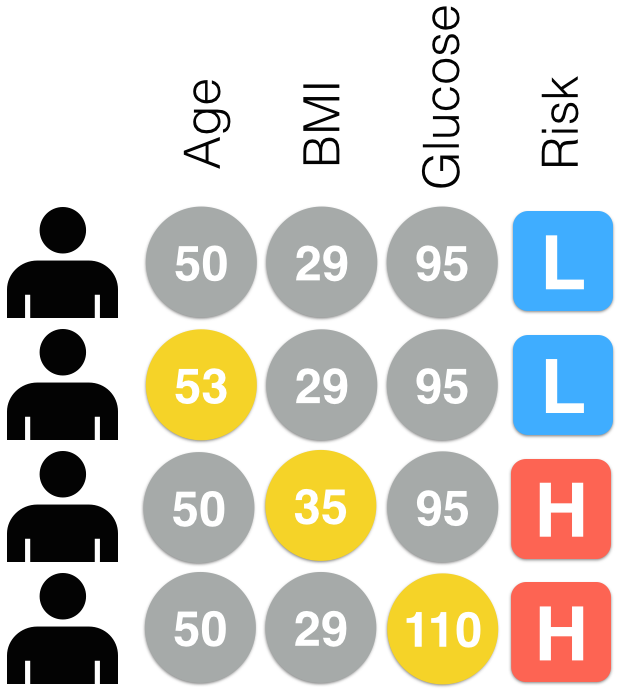
\includegraphics[width=0.3\linewidth]{prospector/local-inspection-explanation} % 0.3
\caption{
This illustration provides an explanation of how local inspection works.  On the top row are the patient's original feature values and the corresponding prediction.  On the bottom three rows, users changed certain values of the patient, highlighted in yellow, and such values impacted the prediction.
}
\label{figs:liexplain}
\end{figure}

Our second core contribution is leveraging our implementation of partial dependence to support the user task of local inspection.  Users can use \prospector to inspect specific data points of interest and see how the models predict how they behave.  In addition, if the users are curious about how a particular data point's risk might change if it had different values, a user can explore this as well.  The idea of localized inspection is illustrated in Figure~\ref{figs:liexplain} using our running example of Diabetes prediction.  At the top, the original patient's feature values are shown, along with the patient's original predicted low risk of having Diabetes. Suppose the analyst was curious to see how the patient's risk would change if his BMI was increased to 35.
Localized inspection allows users to interactively change this value, and see the corresponding prediction.
In order to streamline this kind of exploration we fully compute the
predicted risk for all values of BMI similar to partial dependence.
As seen in Figure~\ref{figs:liexplain} we do this for all features independently
yielding local partial dependence plots for each feature using a single input row.
% Using the idea of partial dependence on a single row of the input data set creates a localized partial dependence describing the axis aligned neighborhood of one point in the prediction function. This enables what-if scenarios by changing some values of the input row and seeing how the predicted outcome changes.

\begin{figure}
\centering
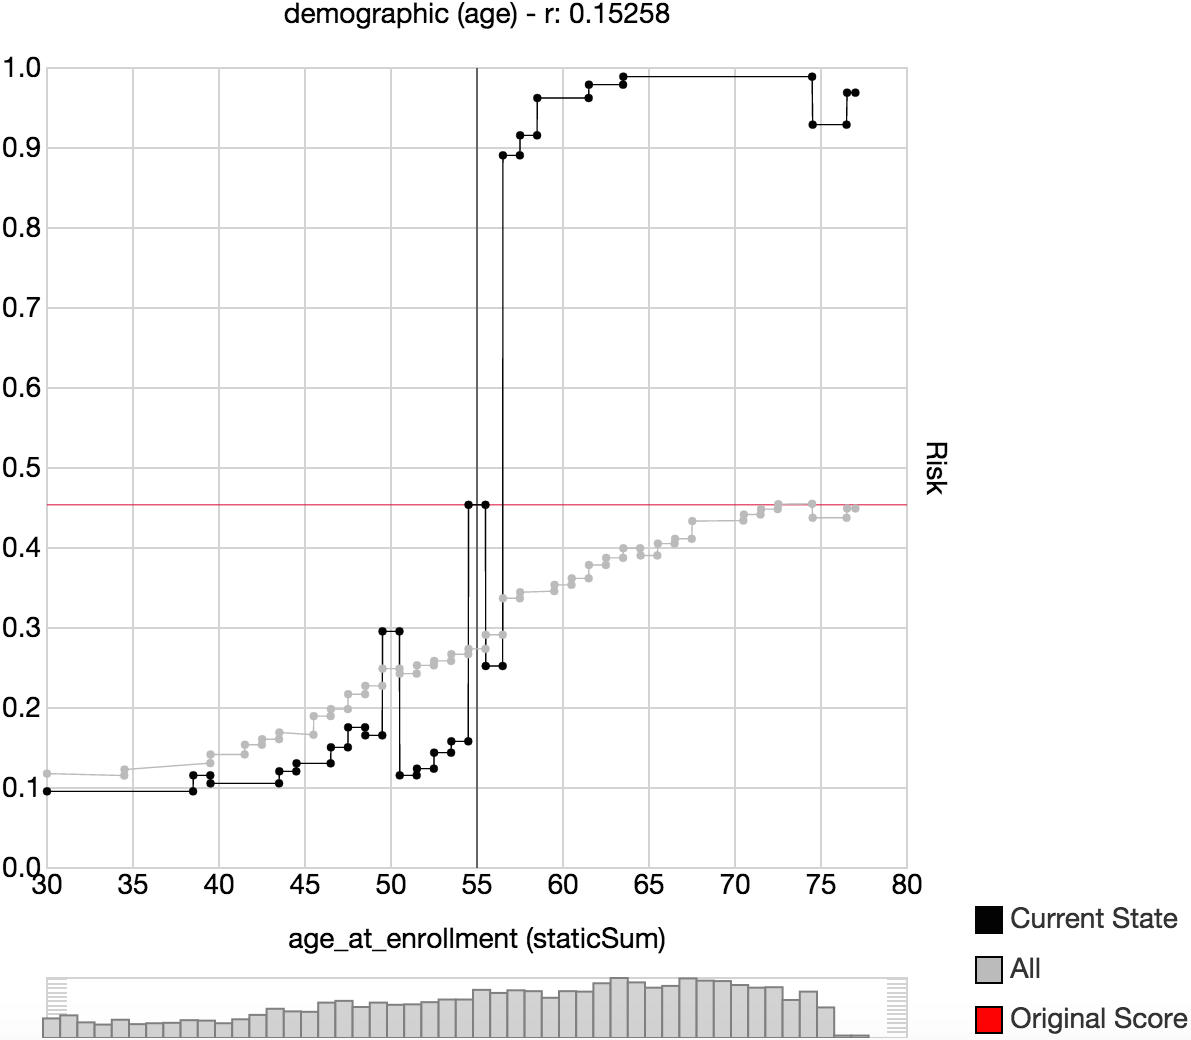
\includegraphics[width=0.8\linewidth]{prospector/compress_1} \\  \vspace*{0.2em} % 0.8 no vs
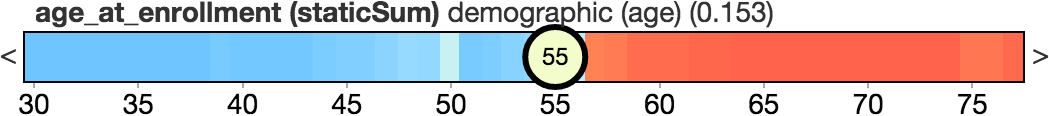
\includegraphics[width=0.9\linewidth]{prospector/compress_2} \\  \vspace*{0.5em} % 0.9 no vs
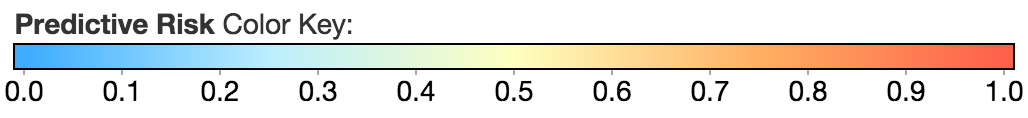
\includegraphics[width=0.7\linewidth]{prospector/color_scale} % 0.7
\caption[The same feature shown as line plot and partial dependence bar.]{
The same feature shown as line plot (top) and partial dependence bar (middle).
Color indicates the predicted risk for the outcome.
The color mapping is shown at the bottom.
}
\label{figs:compress}
\end{figure}

\subsubsection{Partial Dependence Bars}
In order to increase interactivity, encourage exploration, and display a larger number of features at once, we use a novel visual encoding, \emph{partial dependence bars}, a color bar representation of a partial dependence plot, shown in Figure~\ref{figs:compress}. The horizontal axis of a partial dependence bar represents the range of values of a feature, and the color at a given position represents the predicted risk for that value.  Color is mapped to a three-point color scale, where blue represents low risk, yellow represents medium risk, and red represents high risk.  As these bars are meant to aid local inspection, the current feature value of the datapoint being inspected is positioned along the horizontal axis and annotated as a circular label.  Users can drag this circular label left or right to inspect how changes in the feature value affect the predicted risk as well as the local partial dependence of other features.

\subsubsection{Local Feature Importance}
The fourth novel contribution of our research is a technique to simplify the
exploration of the predicted risk space by automatically finding features where a small change in value yields a significantly large change on the predicted risk.

While manipulating values of specific features allows users to test hypotheses on how features of interest may impact the prediction, if users wish to simply understand how to most impact the prediction, manipulating features one-by-one to test impact is an inefficient process.  Instead, \prospector can employ local feature importance, a novel technique that computes the impact of a given feature on the model according to the current values.  This localized feature importance comes in two different flavors: as a feature importance number and as actual suggestions for value changes.

A straight-forward way to define a localized importance of features is to look at the range of possible
predicted risks the feature can create starting from the given data point.
Formula (\ref{eq:importance}) computes the local importance $I$ of a given feature $f$ for the given feature
vector $p$. It sums up the entirety of changes in outcomes for all values $v$ for feature $f$.
The outcome changes are weighted by $\omega$ the likelihood of changing the value from $p_f$ to $v$.
$p^{\ast}$ is the modified feature vector where its value for $f$ is set to $v$ and $pred$ is the prediction function.

\begin{equation}
I_{f}(p) = \int_{-\infty}^{\infty}
\left[ pred(p^{\ast}) - pred(p) \right] \; \omega(v, \, p_f) \; dv
\label{eq:importance}
\end{equation}%
\[
\text{with}\; p^{\ast}_{f} = v \;\text{and}\; p^{\ast}_{g} = p_{g} \;\text{for}\; g \neq f
\]\[
\omega(v, \, p_f) = \frac{1}{\sigma_f \sqrt{2\pi}}
\exp \left( -\frac{(v - p_f)^2}{2\sigma_f^2} \right)
\]

In order for different features to be comparable, $\omega$ takes the distribution of values in the input data
into account. In features with a high spread, a larger change is more likely than in a feature with a narrow value range.
We model the likelihood of the change using a normal distribution with the reference value $p_f$ as mean and the
standard deviation $\sigma_f$ of the observed values of $f$ as standard deviation.
Ordering the features according to this local importance yields features that are likely to
decrease the predicted risk first, then features that have a low impact on the predicted risk,
and finally features that are likely to increase the predicted risk.

% \subsubsection{Local impact suggestions}
Instead of computing local feature importance for all possible changes, it is more
practically useful to compute the importance according to the most \emph{impactful} change for a feature.
An impactful change is the smallest change needed to have the largest change in the predicted outcome.
Note that this is different from the slope of the function since an impactful change
might be after a valley or ridge. Again, in order to have comparable
results, the distribution of values in the input data is taken into account.

\begin{equation}
\argmax_v \left[
s \; \left[ pred(p^{\ast}) - pred(p) \right] \; \omega(v, p_f)
\right]
\label{eq:impact}
\end{equation}

Formula (\ref{eq:impact}) finds the most impactful change of a feature.
$s$ is either $1$ or $-1$ depending on whether to search for the largest increase or decrease.
All other variables are the same as in Formula (\ref{eq:importance}).
The changes yielding the highest impact can be interpreted as suggestions for changing a data point.

\begin{figure}[t]
\centering
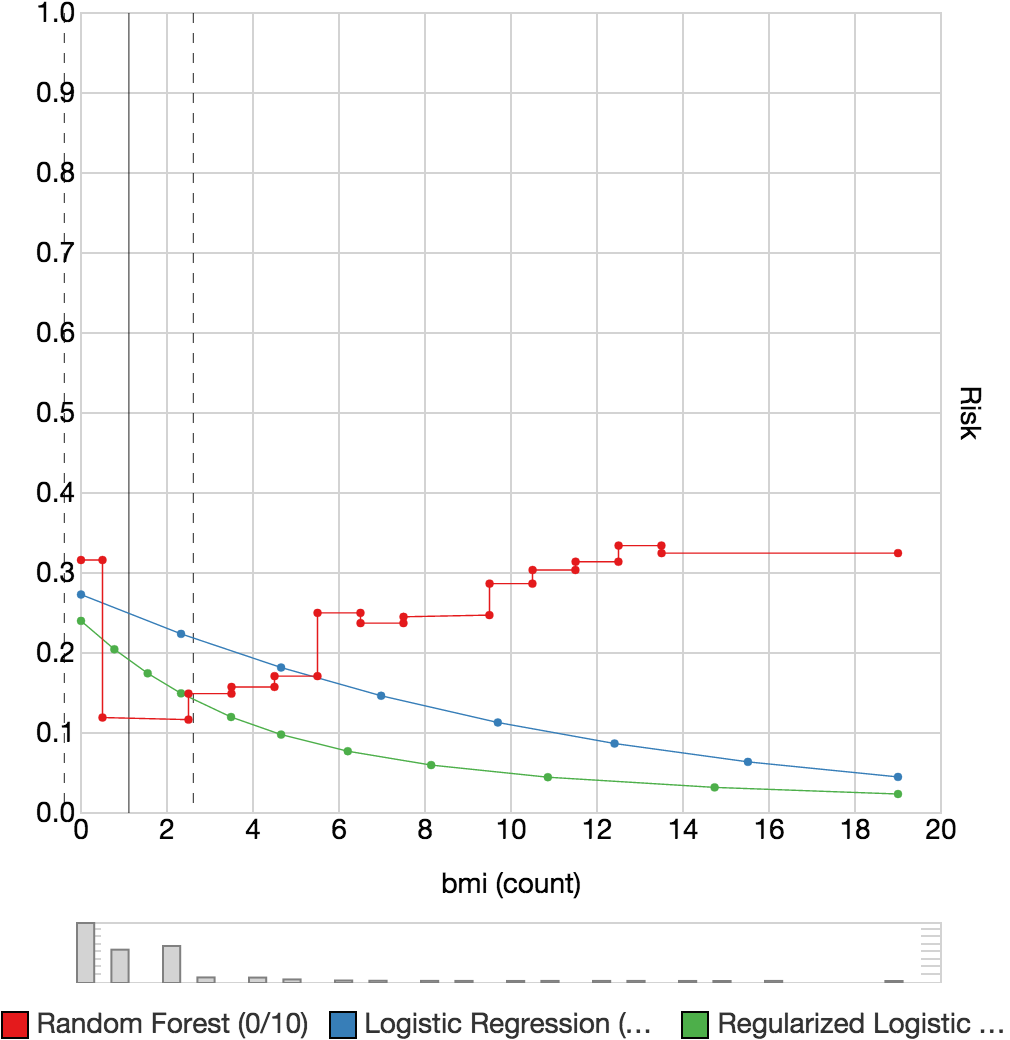
\includegraphics[width=0.7\linewidth]{prospector/cmp_bmi} % 0.8
\caption{
Comparison of three machine learning models on the number of measured BMI values.
The two regression models (logistic regression in blue and regularized logistic regression in green)
can express only a single slope (downwards or upwards) whereas the random forest in red can
model the strong decrease in predicted risk going from no BMI measures to one measure as well as
the later increase again if a patient has several BMI measures.
The random forest is more expressive, but the distribution of input values in the histogram below the plot hint the model might be overfitting as most of the observed values are 2 or less.
}
\label{figs:cmp_bmi}
\end{figure}


\subsubsection{Comparing Multiple Models}

%\joschi{TODO NaN values -- divergent models? there is not much to talk about this here...}

\prospector also supports plotting multiple models in the same plot.  As the input domain and the output range are the same across different machine learning
models on the same data,  partial dependence plots can also be used to compare multiple
models as shown in Figure~\ref{figs:cmp_bmi}.  This is useful for comparing the expressiveness of models and seeing which models are possibly under- or over-fitting the input data.

\subsection{Workflow}

In order to support the workflow of clinical researchers, as described above in the Motivation, \prospector's UI is organized into three main tabs: patient selection, patient inspection, and partial dependence plots.

\subsubsection{Patient Selection}

The patient selection tab allows users to find patients they may want to inspect, based on their ground truth (\eg, whether they actually had Diabetes) and their predicted risk (\eg, assessed likelihood by the predictive model of having the disease).  \prospector provides a visual summary of the patient population by providing a patient selection visualization. The visualization, as seen in Figure~\ref{figs:select}, consists of two columns dividing the population according to their ground truth
(case patients being those actually diagnosed with Diabetes and control patients being not).
Each column is then separated into bins of predicted probabilities in steps of $0.1$
which can be clicked to select the group of patients fitting those criteria.  For instance, if a case patient was predicted with a low risk score, that patient would appear in the top of the right column.  If a bin is too small to provide a clickable area, a box at the side of the column is displayed to allow choosing even small populations.  The selected population is then shown next to the visualization with the individual prediction results shown for each entry.

In order to get more details about patients before selecting, users can hover over a patient in the list and see a summary for the patient, as shown in Figure~\ref{figs:summary}.
In addition to the predicted risk and the ground truth, the interface shows the top 5 most impactful features, for both increasing and decreasing predicted risk, according to the local feature importance described above.  For each impactful feature, the original data value is shown as well as the suggested change and what the resulting predicted risk would be if such a change was made.  This summary provides a preview of how amenable a particular patient's predicted risk is to changing and which features are mostly responsible for their current predicted risk.

\subsubsection{Patient Inspection}

After users select a patient of interest, the UI switches to the
patient inspection tab with the selected patient's data loaded, as shown in Figure~\ref{figs:ui}.
All of the features' partial dependence bars are shown in a scrollable list, with the patient's feature values selected with circular labels.
Users can drag the circular label to change the value of any feature and see the predicted risk change in real-time.
Users can also select a feature and see the corresponding typical partial dependence plot of the feature.
In this plot the local partial dependence of the current patient is shown as
black curve and the global partial dependence of the whole population is shown
in gray. The partial dependence plot is also clickable and users can change the feature value here as well, changing the black vertical line that, in this plot, shows the current value.  

Users can change the order of the partial dependence bars by using the buttons at the top.  In addition to sorting by the feature weight and relevance as determined by the predictive model, users can also sort according to our local feature importance and impactful changes as described above.
If impactful changes are chosen as the order, the suggested changes to each feature are indicated with a white circular label in the partial dependence bar, shown on the bottom left of Figure~\ref{figs:ui}.

Often after analysts have inspected a particular patient, they may wish to find other patients similar to them to see how they react to the predictive model.  If users wish to find patients similar to the one they are inspecting, they can click on the ``Neighborhood" button and \prospector will automatically find the closest patients to the current set of values using feature-wise Euclidean distance.  This similar set of patients are then used as the population in the patient selection tab that users can navigate.

\subsubsection{Partial Dependence Plots}

If users wish to browse the global partial dependence plots of a feature of interest, they can navigate to the third tab.  Users can view multiple models at once by using a combo-box at the top of the user interface to select the models they wish to view in the plot.  Each selected model is assigned a unique color using a quantitative color scale, and a color-coded key is displayed beneath the plot.  If more than one model is selected, the red ``Avg. Score" helper line is not shown.  Users can also filter the global population to a subset population of interest by using a  predicted probability bin or the ``Neighborhood" of a patient in the patient selection tab. This alters the plot accordingly allowing for a more focused analysis for \eg, mispredicted patients, outliers, or patient neighborhoods.

\begin{figure}
\centering
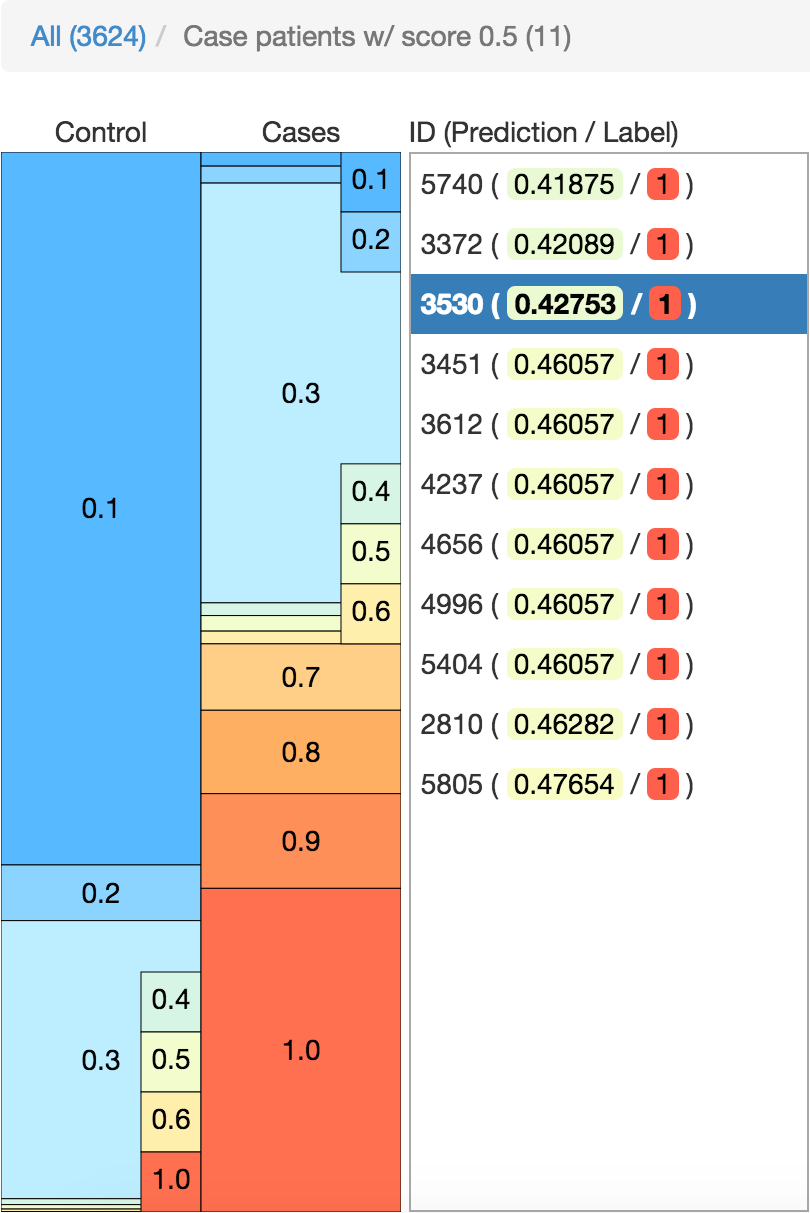
\includegraphics[width=0.5\linewidth]{prospector/patient_select} % 0.6
\caption[The interface for selecting a patient.]{
The interface for selecting a patient.
The left side shows the distribution of patients within different ranges of predicted risk.
The columns indicate the ground truth.
On the right side a list shows the patients of the currently selected range.
}
\label{figs:select}
\end{figure}

\begin{figure}[t]
\centering
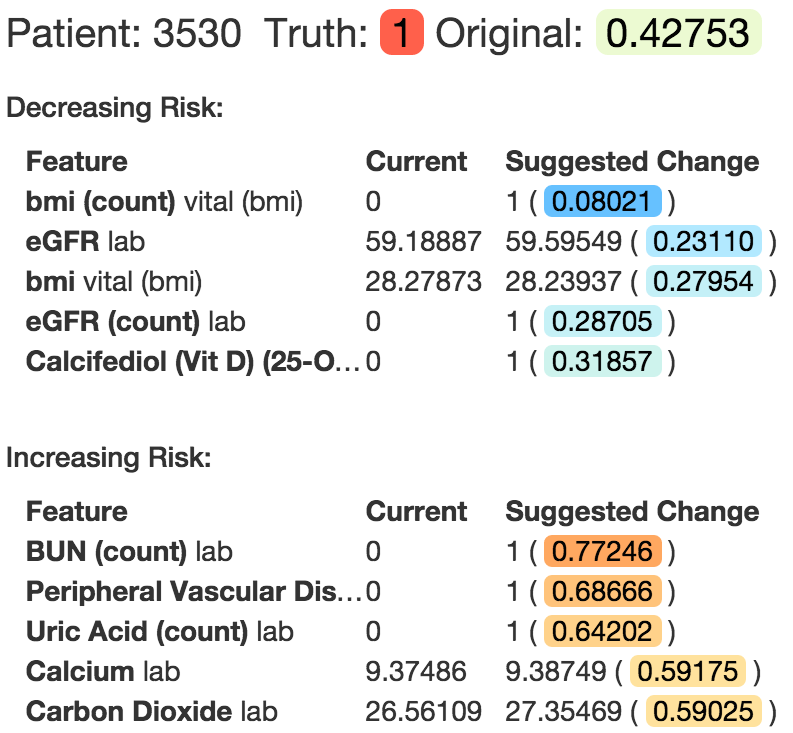
\includegraphics[width=0.5\linewidth]{prospector/patient_summary} % 0.7
\caption{
The summary of one patient. The header line indicates the patient id, the ground truth, and the predicted
risk.
For both decreasing and increasing the predicted risk the top 5 most impactful features are shown.
Each feature shows its current value and the suggested change with the highest impact along with how the predicted risk would change.
}
\label{figs:summary}
\end{figure}

\begin{figure}[t]
\centering
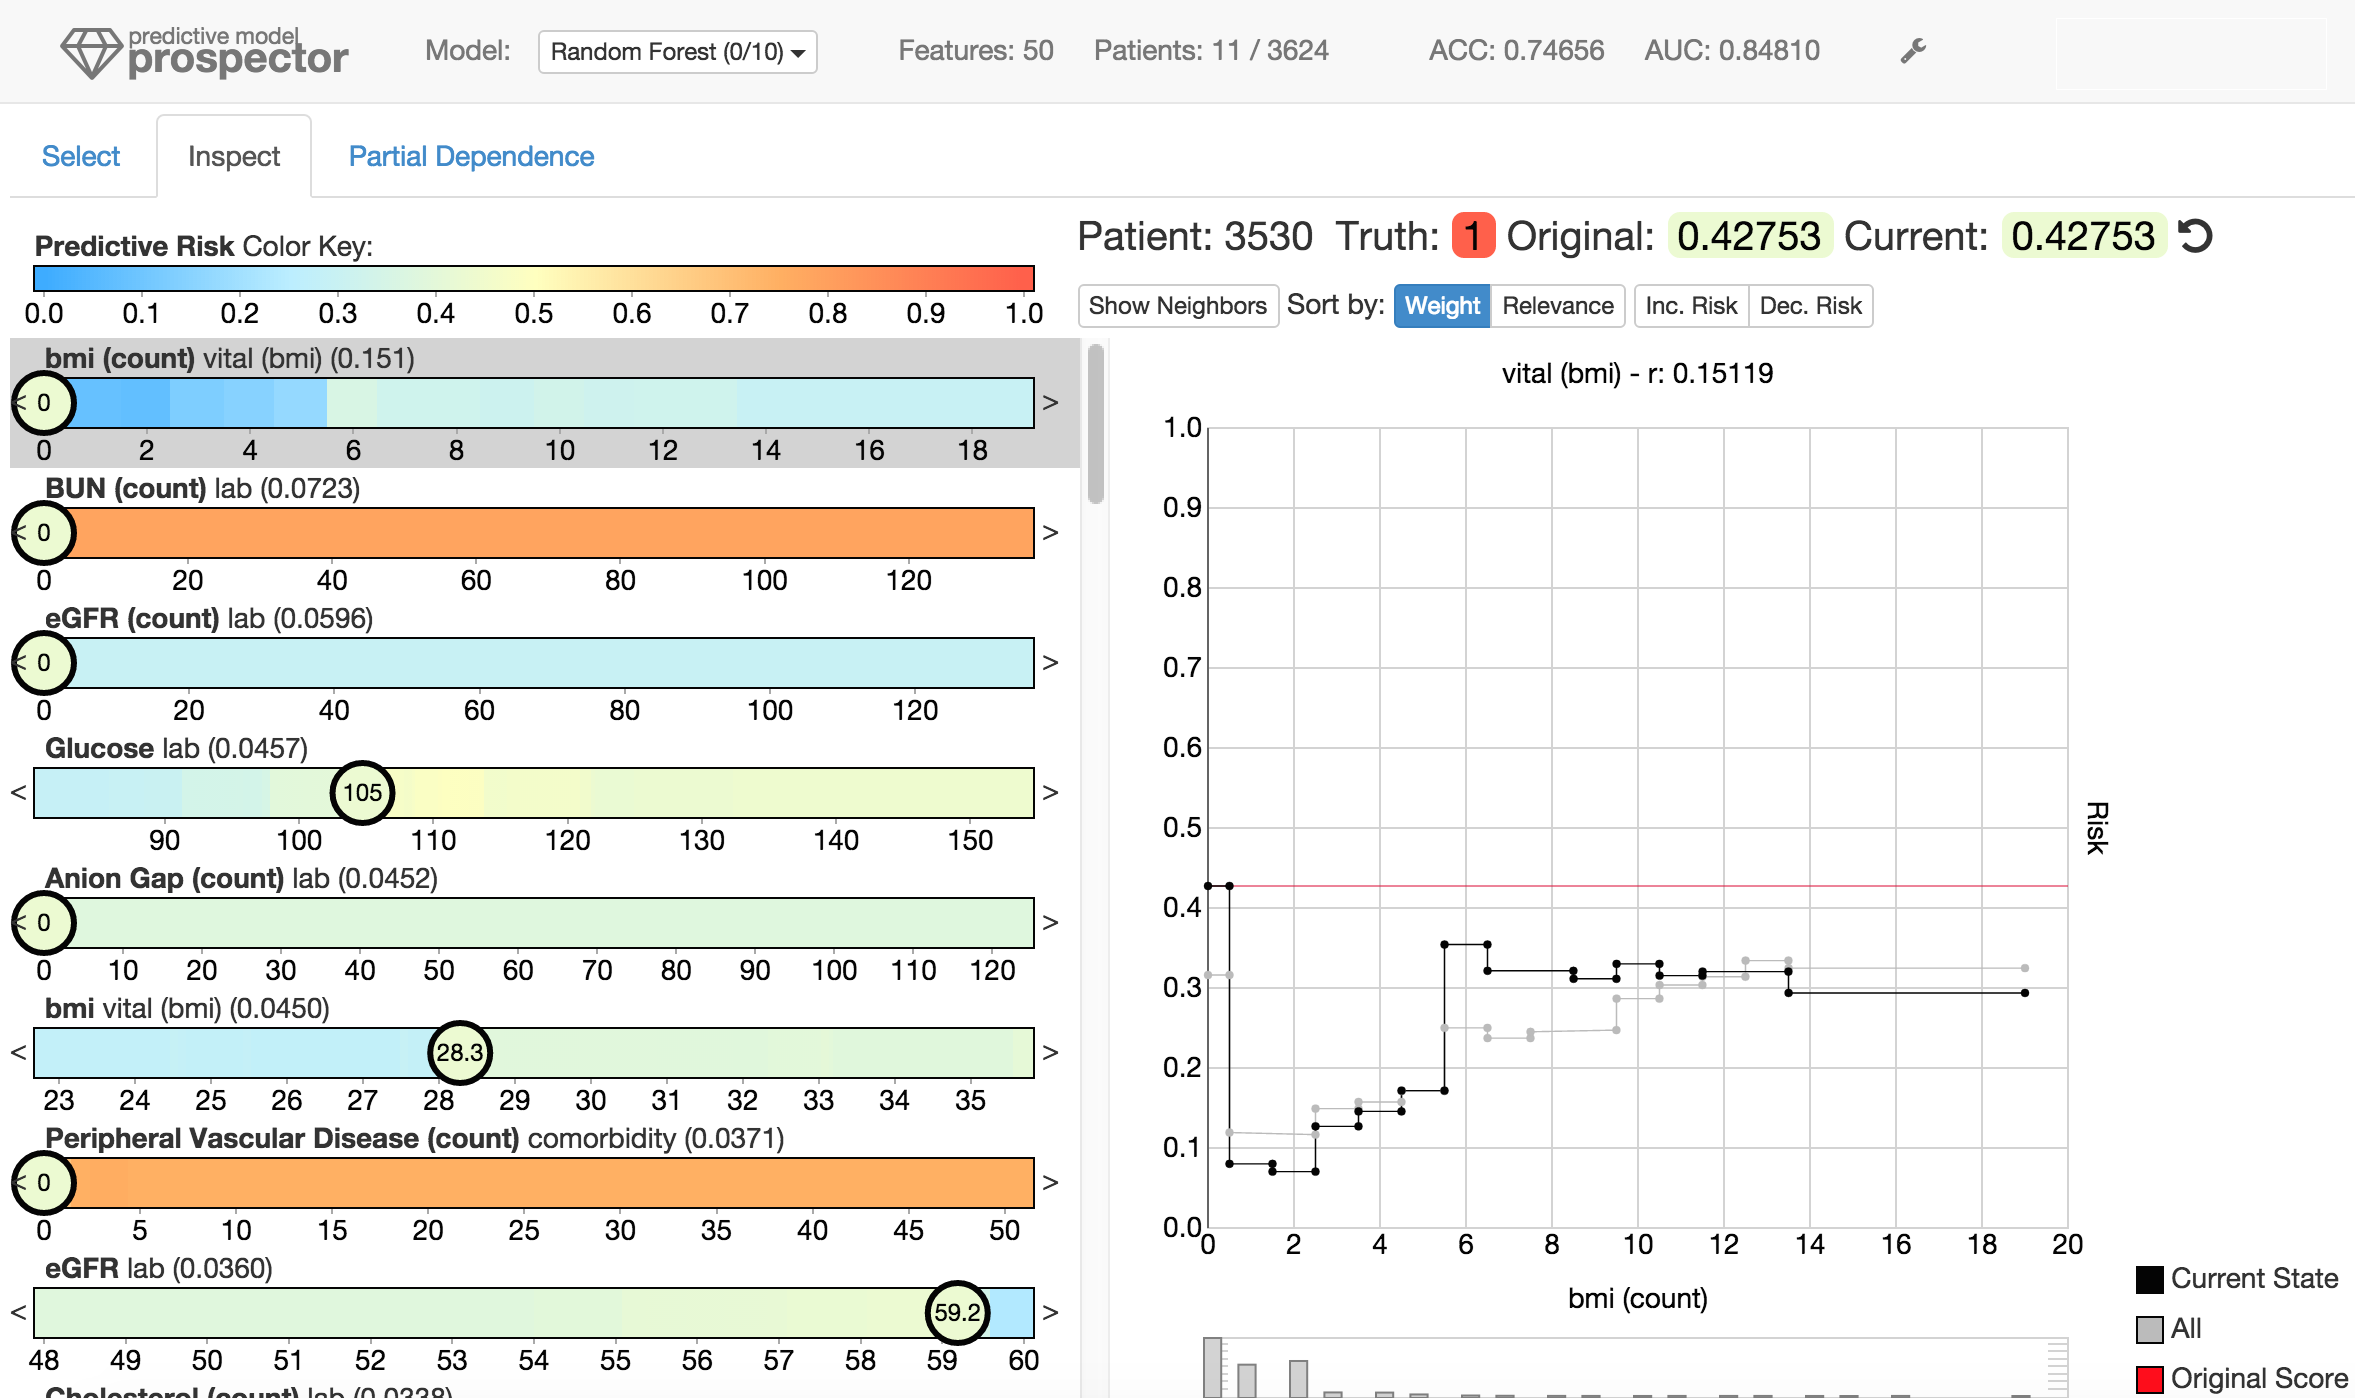
\includegraphics[width=0.8\linewidth]{prospector/ui_inspect} % 0.775
\\
\vspace*{0.75em} % 2
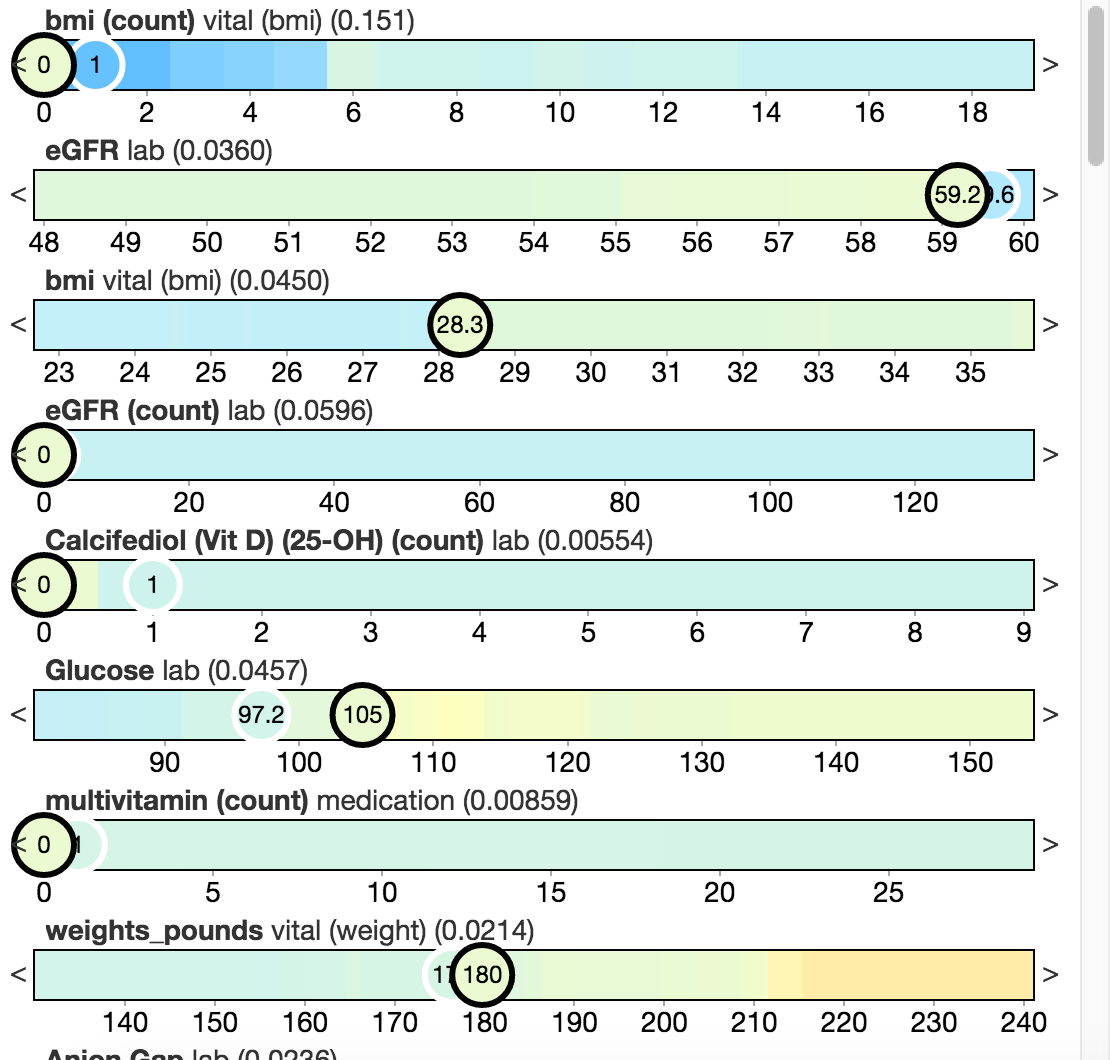
\includegraphics[width=0.3\linewidth]{prospector/ui_sugg} % 0.3
\hspace*{0.2\linewidth} % 18
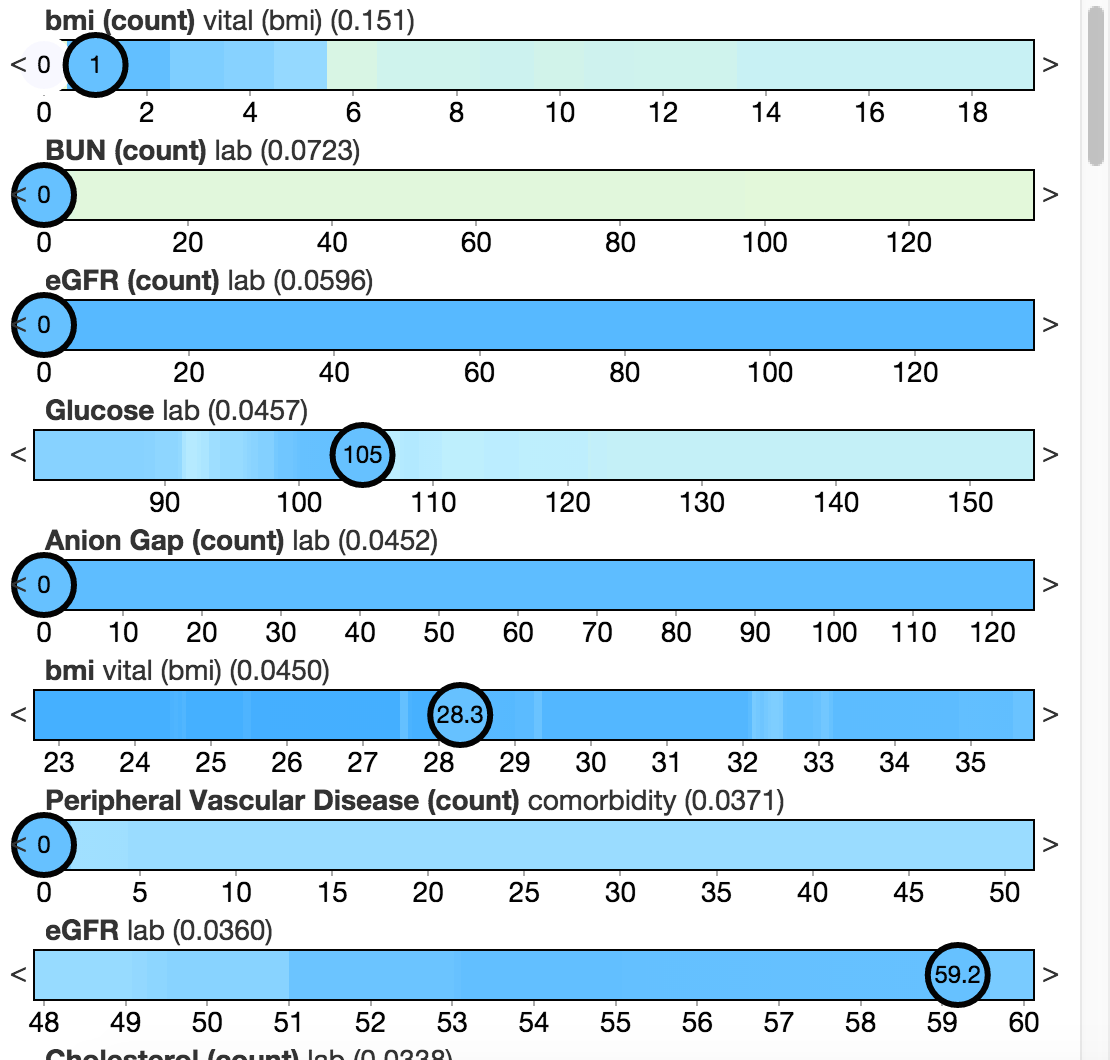
\includegraphics[width=0.3\linewidth]{prospector/ui_change} % 0.3
% \vspace*{1em}
\caption[The user interface of \prospector.]{
The user interface of \prospector is shown at the top.
The bottom left shows suggestions on what changes (white circles) would decrease the
predicted risk the most.
The bottom right shows how the color plots change due to changing a value (namely changing the
bmi value from 0 to 1).
Fully white circles show the original value of the given patient.
}
\label{figs:ui}
\end{figure}
